\documentclass[
paper=a4, % change to a5 if needed
pagesize=auto, 
fontsize=11pt, 
numbers=noendperiod,
headings=twolinechapter, % state the chapter first, then the chapter title
listof=totoc, % add listo of figures and tables to toc
bibliography=totoc % add bilbiography to toc
]
{scrbook}
% --------
% Bibliography
% --------
\usepackage[
style=authoryear, % other styles available
backend=biber, % you will have to set biber as your backend in TeXstudio
maxnames=2, % display maximum two authors
]
{biblatex}
\addbibresource{refs.bib} % tell latex where the references are stored
% --------
% Additional packages
% --------
\usepackage{lipsum} % for blind text only
\usepackage[hidelinks]{hyperref} % for internal links, such as Table of content (toc), figures and references
\usepackage{graphicx} % for the integration of figures
\graphicspath{{figures/}} % set absolute path to figures
%\usepackage{import}
\usepackage{svg}
\svgpath{{figures/}} % tell the svg package where to find the svg files
\usepackage{floatrow} % for global setting of fontsize in floats (tables and figures)
\floatsetup[figure]{font={footnotesize}}
\usepackage{booktabs} % for nicer tables
% --------
% Glossaries
% --------
\usepackage[record,style=indexgroup]{glossaries-extra}
\setabbreviationstyle[acronym]{long-short}
% acronyms
\GlsXtrLoadResources[src=source/acronyms,sort=letter-nocase,group=Acronyms]
% notations
\GlsXtrLoadResources[src=source/notations,sort=letter-nocase,group=Notations]
% symbols
\GlsXtrLoadResources[src=source/symbols,sort=letter-nocase,group=Symbols]
% rename the chapter from GLossary to Nomenclature
\renewcommand*{\glossaryname}{Nomenclature}
%
% --------
% Even more additional packages
% --------
\usepackage{csquotes}
\usepackage{siunitx}
\usepackage{cleveref}
\usepackage{enumitem}
% --------
% Penalties
% --------
\widowpenalty=100000
\clubpenalty=100000
\displaywidowpenalty=100000
% --------
% Bib filters
% --------
\DeclareSourcemap{
	\maps[datatype=bibtex]{
		% remove fields that are always useless
		\map{
			\step[fieldset=abstract, null]
			\step[fieldset=pagetotal, null]
			\step[fieldset=month, null]
		}
		% remove URLs for types that are primarily printed
		\map{
			\pernottype{software}
			\pernottype{online}
			\pernottype{report}
			\pernottype{techreport}
			\pernottype{standard}
			\pernottype{manual}
			\pernottype{misc}
			\step[fieldset=url, null]
			\step[fieldset=urldate, null]
		}
		\map{
			\pertype{inproceedings}
			\pertype{article}
			% do not show ISBN or ISSN for proceedings and journal papers
			\step[fieldset=isbn, null]
			\step[fieldset=issn, null]
		}
		\map{
			\pertype{book}
			\pertype{inbook}
			\pertype{incollection}
			% do not show DOI for books
			\step[fieldset=doi, null]
		}
	}
}
%\includeonly{source/introduction.tex}
\begin{document}
% --------
% Ttilepage
% --------
\titlehead{Some University
		\hfill WS~2022/2023\\
	School of Something\\
	University Street 100\\
	12345 City}
\subject{Dissertation}
\title{Thesis Title}
\subtitle{Subtitle}
\author{John Doe}
\date{30. February 2022}
\publishers{\begin{tabular}{lll}
			&Chair: & Prof. A \\
			&First Examinor: & Prof. B\\
			&Second Examinor: & Prof. C
			\end{tabular}
			}
\dedication{Dedication}
\maketitle
% --------
% Preface
% --------
\frontmatter % switches to lower case roman page numbers
\tableofcontents
\listoffigures
\listoftables
\printunsrtglossaries
% --------
% Content
% --------
\mainmatter % switches to latin page numbers
\chapter{Introduction}%
\label{ch:introduction}%
Using \verb|\parencite| produces a reference in parentheses, for example \parencite{bishopPatternRecognitionMachine2006}. In contrast, using \verb|\textcite| produces a reference without parentheses, for example \textcite{rumelhartLearningRepresentationsBackpropagating1986}. 	

\lipsum%
%
\section{Motivation}%
\label{sec:motivation}%
\lipsum%
\begin{figure}
	\centering
	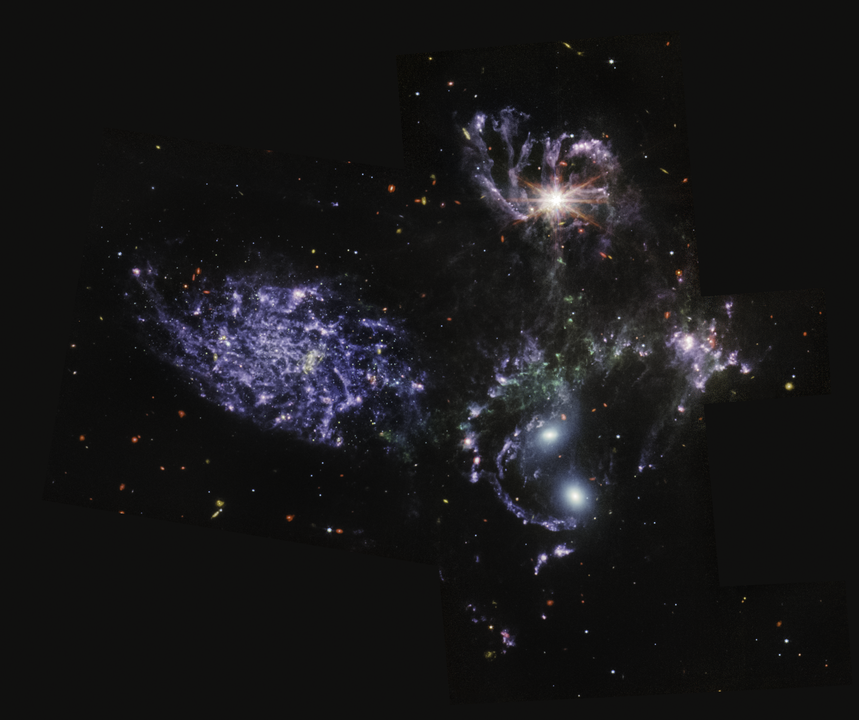
\includegraphics{jamesWebb}
	\caption[James Webb Stephan's Quintet]{Image of the Stephan's Quintet recorded by the James Webb telescope}
	\label{fig:jamesWebb}	
\end{figure}
%
\section{Objectives}%
\label{sec:objectives}%
\lipsum%
%
\section{csquotes package}%
\label{sec:csquotes}
With \verb|\enquote| a simple quotation can be displayed inline, for example \enquote{A short quote.} In contrast, using \verb|\blockquote| will display larger quotes as a separate block: \blockquote[\cite{bishopPatternRecognitionMachine2006}, p.~1]{The problem of searching for patterns in data is a fundamental one and has a long and successful history. For instance, the extensive astronomical observations of Tycho Brahe in the 16th century allowed Johannes Kepler to discover the empirical laws of planetary motion, which in turn provided a springboard for the development of classical mechanics. Similarly, the discovery of regularities in atomic spectra played a key role in the development and verification of quantum physics in the early twentieth century. The field of pattern recognition is concerned with the automatic discovery of regularities in data through the use of computer algorithms and with the use of these regularities to take actions such as classifying the data into different categories.}
%
\section{siunitx package}%
\label{sec:siunitx}
A quantity can be displayed using \verb|\qty[<option>]{<number>}{<unit>}|, for example \qty{9.81}{\meter\per\second\squared}. The units can be formatted differently by setting a specific option. For example, by adding the option \verb|per-mode = symbol|, the quantity is displayed as \qty[per-mode = symbol]{9.81}{\meter\per\second\squared}. In contrast, by adding the option \verb|per-mode = faraction|, the quantity is displayed as \qty[per-mode = fraction]{9.81}{\meter\per\second\squared}.

Other features include the \verb|\qtylist{<numbers>}{<units>}| command for a list of quantities, such as \qtylist{1; 2; 3}{\meter}, and the \verb|\qtyrange{<start>}{<stop>}{<units>}| command for a range of quantities producing \qtyrange{1}{4}{\meter}.
%
\section{cleveref package}%
\label{sec:cleveref}
With the cleveref package, cross-referencing to \cref{fig:jamesWebb} or \cref{ch:introduction}, for example, becomes more convenient. The reference is integrated using the \verb|\cref{<label>}| command. When the number of the referenced object changes, cleveref will notice that and handle the update of all references. 

Note, that the object that should be cross-referenced needs a label. For example, \cref{fig:jamesWebb} has the label \verb|\label{fig:jamesWebb}|.

If the referenced objects should be capitalized, the \verb|\Cref{<label>}| command can be used. \Cref{fig:jamesWebb}, for example, is at the beginning of a sentence and should be capitalized. 
%
\section{enumitem package}%
\label{sec:enumitem}
With the enumitem package, custom labels for lists are enabled. For example:
\begin{enumerate}[leftmargin=*, align=left,start=1,label={\bfseries L\arabic*}]%
	\item \lipsum[0-1]
	\item \lipsum[0-1]
	\item \lipsum[0-1]
\end{enumerate}
%
\section{bib2gls and glossaries-extra packages}%
\label{sec:gls}
With the \verb|\gls{<label>}| command, an abbreviation, a symbol or an example notation can be displayed. For example, the first time derivative can be denoted as \gls{x_dot} and acronyms such as \gls{ml} or \gls{dl} can be handled automatically. When \gls{ml} is called for the second time, only its acronym is displayed. Also, plural terms are possible with the \verb|\glspl{<label>}| command, so that several \glspl{fft} are displayed in plural. Exemplary use for notations and symbols could be the following: the determinant of matrix $X$ can be denoted as \gls{determinant} and the angular velocity can be denoted as \gls{omega}. 

\section{Integrating vector graphics}%
\label{sec:svg}
\lipsum[0-3]
\begin{figure}
	\centering
	\includesvg{plot}
	\caption{A sample vector graphic}
	\label{fig:plot}
\end{figure} 	

\chapter{Results}%
\label{ch:results}%
\lipsum%
\section{First Results}%
\label{sec:results1}%
\lipsum%
\begin{table}
	\centering
	\begin{tabular}{@{}lll@{}}
		\toprule
		experiment & model   & error \\ \midrule
		1        & awesome model & 2       \\
		2        & even better model & 0.1       \\ \bottomrule
	\end{tabular}
	\caption[Results]{Overview of the results}
	\label{tab:results}	
\end{table}
\section{Second Results}%
\label{sec:results2}%
\lipsum%
\chapter{Conclusions}%
\label{ch:conclusions}%
\lipsum%
\section{Limitations}%
\label{sec:limitations}%
\lipsum%
\section{Outlook}%
\label{sec:outlook}%
\lipsum%
% --------
% Appendix
% --------
\appendix%
\chapter{Further Details}%
\label{ch:appendix}
\lipsum%
% --------
% Bibliography
% --------
\backmatter % chapters are not numbered anymore
\printbibliography%
\end{document}